\chapter{Plugins}
\label{chap:modulos}

In this chapter a general description about the plugins that are availables in
the {\lpmd} code. Some properties related to each plugin, examples and for some
cases a theoretical analysis of the capabilities availables for the plugin.
More examples related to the program {\lpmd} and how to use it, are availables
in the chapter~\ref{chap:exa}.

The plugins are divided for type in the followging sections. The goal of this
chapter is maintain a updated references about each module. Neverthless the
more updated information, including bugs and new features are available online
in \url{http://www.lpmd.cl}.

%%%%%%%%%%%%%%%%%%%%%%%%%%%%%%%%%%%%%%%%%%%%%%%%%%%%%%%%%%%%%%%%%
%%%%%%%%%%%%%%%%%%%%%%%%%%%%%%%%%%%%%%%%%%%%%%%%%%%%%%%%%%%%%%%%%
\section{Input/Output Plugins}
\label{chap:modulos:entradasalida}

This plugins are used with the \verb|input| and \verb|output| options. The
module name and all the options related to the module are set in the same line.
The general form to use this plugins is :

\control{input module=mod file=.. opc1=.. ...  opcN=...}
\control{output module=mod file=.. opc1=.. ... opcN=...}

\noindent
where the \verb|opcX| are the option related to each plugins, \verb|file|
correspond to the file to be load or writed and \verb|module| correspond to the
name of the plugin that will be used.

\subsection{dlpoly}

This plugin, is used to read and write file of the type \verb|HISTORY| and
\verb|CONTROL| related to the \verb|dl_poly| software. The options availables
in the \verb|dlpoly| plugin are :


\fb{
\begin{tabular}{lcl}
 file & = & Input/Output file name.\\
 level & = & File level (0,1,2).\\
 preiodicity & = & Set the periodicity \textit{key}\\
 &&of a CONFIG file.\\
 ftype & = & Indicate the type of file, \texttt{HISTORY} or\\
 &&\texttt{CONFIG} are valid variables.\\
\end{tabular}
}

A example of how to use this plugin for input output could be found in,
\url{http://www.lpmd.cl/Plugins/doku.php?id=plugins:in_out#dlpoly}.

\subsection{lpmd}\label{subsec:lpmdformato}

Is a particular format used in the {\lpmd} software. Between the advantages of
this format is that save additional information to the atomic position. With
this format the cell properties are stored in each configuration, and
additional information about atomic tags can be saved too. In this particular
format the atom position are stored in fractional coordinated. Three diferent
levels are available, 0 save/read positions only, 1 save/read positions and
velocity and level 2 is similar to the level 1, but this save the acceleration
of the atoms.

This plugins also can read and write in compress format \verb|zlp| that is a
lpmd format compressed using the zlib. Between the options available with this
plugins are :

\fb{
\begin{tabular}{lcl}
 file & = & Input/Output filename.\\
 level & = & Set the file level, the valid values are, \\
           &&0(pos),1(pos y vel) y 2(pos,vel y ace).\\
 extra & = & Additional information about the atoms tags, \\
           &&rgb, type, etc.\\
 type & = & Specify the type of file, \texttt{lpmd}(default) or \\
           &&\texttt{zlp}.\\
 blocksize & = & Size of the compression\textit{block}, when\\
           &&type is \texttt{zlp}.\\ 
\end{tabular}
}

A simple example of using the plugin \verb|lpmd| :

\begin{itemize}
 \item \textbf{Loading a lpmd file}
       \control{input module=lpmd file=archivo.lpmd}
 \item \textbf{Writing a lpmd file with velocities}
       \control{output module=lpmd file=salida.lpmd level=1}
\end{itemize}

More examples can be found in
\url{http://www.lpmd.cl/Plugins/doku.php?id=plugins:in_out#lpmd}.

\subsection{vasp}

This plugin is used to read \verb|POSCAR| files from \verb|vasp| software. This
type of files(\verb|POSCAR|) have information about the atomic positions and
the cell size. However is \textbf{very important} highlight that this plugin
need information about the atoms species in the right order, i.e. the option
\verb|species| of this plugins have to be correctly assigned, in order to can
have a good interpreation of the cell.

\fb{
\begin{tabular}{lcl}
 file & = & Input file name\\
 species & = & List of all the species (oredered) of \\
 &&the POSCAR file.\\
 level & = & Indicate the level of the file.\\
 type & = & Type of positions of the atoms, Direct/Cartesian.\\
\end{tabular}
}

Examples about how to use the vasp plugin, can be found in
\url{http://www.lpmd.cl/Plugins/doku.php?id=plugins:in_out#vasp}.

\subsection{xyz}

The \verb|xyz| is one of the more classical format file used in different areas
of research, in particular molecular dynamics that is our case. This plugin is
used to read and write the \verb|xyz| filetypes. Between the current option for
this format we have :

\fb{
\begin{tabular}{lcl}
 file & = & Input/Output filename.\\
 level & = & Set the level of the file, available values are \\
           &&0(pos),1(pos y vel) y 2(pos,vel y ace).\\
 coords & = & Used to read/write cells that are centered in the origin \\
           &&or centered in the positive region of the coordinates axes \\
           &&available valid values are: centered/uncentered.\\
 inside & = & The values are true/false, Set if the atoms outside of the \\
          &&cell must to be rellocated.\\
 external & = & Values are ignore/consider. Indicate if you want ignore or \\
          &&considerar the atoms that are located outside the cell.\\
\end{tabular}
}

Many of this options are not frequently used in a {\lpmd} simulation. However
that can be useful when you need work with utilties like lpmd-analyzer or
similars. A general idea of how to use this plugin is :

\begin{itemize}
 \item \textbf{Loading a xyz file}
       \control{input module=xyz file=archivo.xyz}
 \item \textbf{Writing in a xyz file with atom velocities}
       \control{output module=xyz file=salida.xyz level=1}
\end{itemize}

Like in all the plugins, not all option are necessary, most of them have
default values. More examples about this plugin could be found in
\url{http://www.lpmd.cl/Plugins/doku.php?id=plugins:in_out#xyz}.

\subsection{mol2}

This plugin is used to read and write \verb|mol2| file types. Is imperative
highligh that this support is only partial, the developers do not work more in
this plugins have only small frequently updates. However this, could be useful
in some particular cases. The options availables for this plugin are :

\fb{
\begin{tabular}{lcl}
 file & = & File that have the atomic configurations.\\
\end{tabular}
}

Althought it is a basic support, the write process had been show good
performance. Examples of how to use this plugin can be found in
\url{http://www.lpmd.cl/Plugins/doku.php?id=plugins:in_out#mol2}.

\subsection{pdb}

This plugin is used to read an write \verb|pdb| file types. In a similar way
that for the case of the \verb|mol2| plugin, the \verb|pdb| plugin is partially
supported. However you can use for basic read and write of \verb|pdb| files.
Between the principal options of this plugins are :

\fb{
\begin{tabular}{lcl}
 file & = & Input/Output file in pdb format.\\
\end{tabular}
}

Examples of how to use this plugins can be found in
\url{http://www.lpmd.cl/Plugins/doku.php?id=plugins:in_out#pdb}.

\subsection{rawbinary}

The \verb|rawbinary| plugin has been developed in order to improve the
performance of read and write files when the size of the information is
considerably big (orders of Gigabytes). This is used for read/write of a binary
file (\verb|raw|). The goal of use this format is improve the performance of
analysis and similars. Between the option associated to thisplugins are :

\fb{
\begin{tabular}{lcl}
 file & = & Input/Output file name.\\
 level & = & Level of the file.\\
\end{tabular}
}

Is important highlight that this format only store the atom positions
(velocities and acceleration, depending of the level) and information about the
cell. Examples of how to use this plugins can be found in
\url{http://www.lpmd.cl/Plugins/doku.php?id=plugins:in_out#rawbinary}.

%%%%%%%%%%%%%%%%%%%%%%%%%%%%%%%%%%%%%%%%%%%%%%%%%%%%%%%%%%%%%%%%%
%%%%%%%%%%%%%%%%%%%%%%%%%%%%%%%%%%%%%%%%%%%%%%%%%%%%%%%%%%%%%%%%%
\section{Cell generators plugins}
\label{chap:modulos:generadores}

This plugins are load by the \verb|input| option. The options related to the
plugins have to be assigned in the same line. A general idea of how to use this
kind of plugins is :

\control{input module=mod opc1=.. ...  opcN=...}

\noindent
where \verb|opcX| are the options of each particular type of plugin. This kind
of plugins only \textit{generate} simulation cells (do not can be used in the
\verb|output| option). The goal of this kind of plugins is try to help to the
users to generate easy types of structures with less work. All these kind of
plugins will be explained detailed now.

\subsection{crystal3d}
This plugin is used to build 3D critaline strctures. This plugins is used
\textit{instead} of an input file. Between the princial options allowed for
thid plugins are :

\fb{
\begin{tabular}{lcl}
 symbol & = & Atomic symbol of the atom.\\
 n$\alpha$ & = & $\alpha=x,y,z$ Number of repetitions in each direcition.\\
 type & = & Kind of cell, the vailables values are fcc, bcc, hcp and sc.\\
\end{tabular}
}

For example if we want to generate a cubic cell of \textbf{Fe} with a size of
10 \AA for every axes, we will use :

\begin{itemize}
 \item \textbf{Put the cell details}
       \control{cell crystal a=10 b=10 c=10 alpha=90\textbackslash beta=90
gamma=90}
 \item \textbf{Generate the atoms fcc inside the cell}       
       \control{input module=crystal3d type=fcc symbol=Fe\textbackslash nx=3
ny=3 nz=3}
\end{itemize}


With this we generate a cristaline cell of the \verb|fcc| type using a network
parameter $ a = 10/3 = 3.33$, to start our simulation.

\subsection{crystal2d}

This plugin is used to generate crystals in 2D. The options available in this
plugin are :

\fb{
\begin{tabular}{lcl}
 symbol & = & Atomic symbol of the specie.\\
 a & = & Long of the base vector $\vec{a}$.\\
 b & = & Long of the base vector $\vec{b}$.\\
 gamma & = & angle between the vectors.\\
 n$\alpha$ & = & $\alpha=x,y$ The inverse on the crystal long.\\
\end{tabular}
}

Using as an example, a two dimensional triangular network with Ar atoms, wehere
the size of the crystal is 10 \AA.

\begin{itemize}
 \item \textbf{Set the cell details}
       \control{cell crystal a=10 b=10 c=0 alpha=90 beta=90 gamma=90}
 \item \textbf{We put the atoms inside the crystal}
       \control{input module=crystal2d a=2 b=2 symbol=Fe gamma=60\textbackslash 
        nx=2 ny=2}
\end{itemize}

With this we generate a 2D crystal. More examples could be found in
\url{http://www.lpmd.cl/Plugins/doku.php?id=plugins:cell_generators#crystal2d}.

\subsection{voronoi}
This plugin use the \textbf{voronoi} contruction to generate nanostructures of
materials. The principal options avilables for this plugins are :

\fb{
\begin{tabular}{lcl}
 symbol & = & Atomic symbol of the specie.\\
 type & = & Set the cristaline grain, fcc, bcc, etc.\\
 a & = & Network constant of the cristal.\\
 grains & = & Number of grains inside the cell.\\
\end{tabular}
}

Similar to the previous showed cell generators plugins, the general information
of the cell is assigned in the \verb|cell| option. Instead, the part associated
to the plugins is assigned in the \verb|input| section. However all this, we
will use now a different example, using directly the command line (quick-mode)
to generate the nanostructure. In a single terminal execute :

\begin{verbatim}
 lpmd-visualizer -i voronoi:symbol=Fe,type=fcc,a=3.62,grains=6 -u lpvisual -L 
 50,50,50
\end{verbatim}

\begin{figure}[h!]
 \centering
 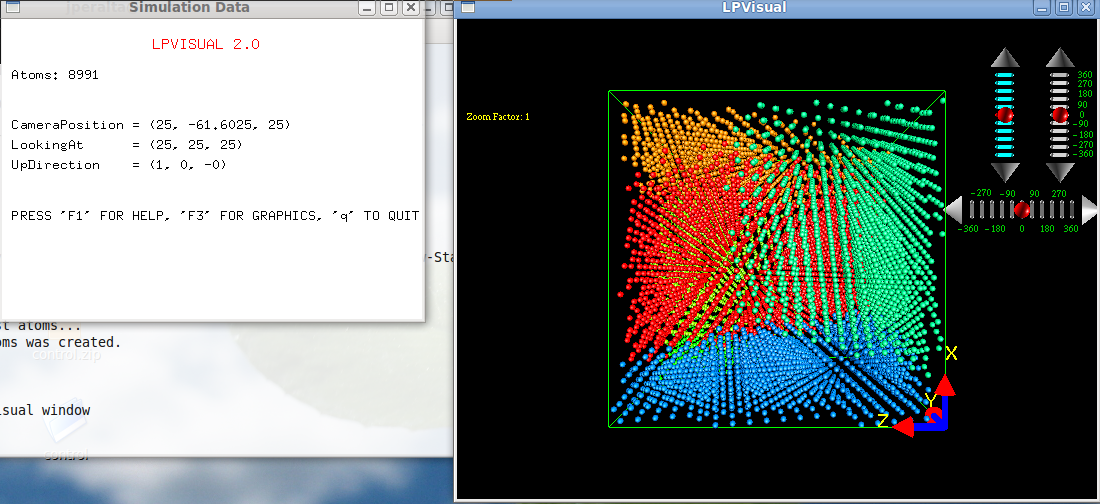
\includegraphics[scale=.35]{voronoi-1.png}
 \label{fig:voronoi-1}
 \caption{Screenshoot of \texttt{lpmd}. This use lpvisual to show the cell
generated using skewstart.}
\end{figure}

If you don't want to use or do not have installed lpvisual remove the option
\verb|-u lpvisual| from the command line and define some output to save this
configuration, for example \verb|-o xyz:file=output.xyz|. The results of the
quick-mode method are showed in the figure~\ref{fig:voronoi-1}. For the case
that you want to save this cell and visualize (using lpvisual), you will need
to execute in this way :

 \begin{verbatim}
 lpmd-visualizer -i voronoi:symbol=Fe,type=fcc,a=3.62,grains=6 \
 -u lpvisual -L 50,50,50 -o lpmd:file=new.lpmd,extra=rgb
\end{verbatim}

\subsection{skewstart}
This method was developed by \textit{K. Refson} for the molecular dynamics code
\textbf{moldy}. The goal of this method is build a atomic configuration
non-periodic and highly regular in order to guarantee a minimal space between
the atoms. The options availables in this plugin are :

\fb{
\begin{tabular}{lcl}
 symbol & = & Atomic symbol of the specie.\\
 atoms & = & Set the number of atoms inside of \\
 &&the cell.\\
\end{tabular}
}

As an example of how to use this plugin, consider a argon cell of 108 atoms in
a cell of size 20 \AA~. For this :

\begin{itemize}
 \item \textbf{Set the cristal details}
       \control{cell crystal a=20 b=20 c=20 alpha=90 beta=90 gamma=90}
 \item \textbf{Build the atoms positions using skewstart method}
       \control{input module=skewstart symbol=Ar}
\end{itemize}

Other examples can be found in
\url{http://www.lpmd.cl/Plugins/doku.php?id=plugins:cell_generators#crystal2d}.


%%%%%%%%%%%%%%%%%%%%%%%%%%%%%%%%%%%%%%%%%%%%%%%%%%%%%%%%%%%%%%%%%
%%%%%%%%%%%%%%%%%%%%%%%%%%%%%%%%%%%%%%%%%%%%%%%%%%%%%%%%%%%%%%%%%
\section{Cell managers plugins}

This plugins are responsable to generate the \textbf{smart lists} to realize
molecular dynamics simulation and/or analysis of atomic structures. This
\textbf{smart lists} help to reduce the calculation time during a process. The
scheme and extra information about this type of \textbf{cell-managers} could be
found in the work of Davis et al~\cite{Davis2010}.

\subsection{linkedcell}
This is the standard linkedcell list method, is one of the more fast and more
used method in Molecular dynamics. The improve for a large number of atoms is
huge in comparison with different types like minimumimage and is the most used
in defferent MD codes. This model generate subdivisions of the cell in the
different directions of the structure cell, is important keep in mind that the
subdivision size are minor that the minimum interaction distance between the
particles (related to the specific potential). However this, the plugin have an
auto-mode in order to make an automaic cell division.

\begin{itemize}
 \item \textbf{Loading the plugin}
       \control{use linkedcell \\ cutoff 2.0 \\ nx 10\\ ny 10\\ nz 10\\enduse}
 \item \textbf{Loading the plugin} \texttt{auto}.
       \control{use linkedcell \\ cutoff 2.0 \\ mode auto\\enduse}
 \item \textbf{Applying the plugin}
       \control{cellmanager linkedcell}
\end{itemize}

\subsection{minimumimage}
This plugin use the minimum-image model to realize the atomic interaction
process. Is frequently more slow, and only need the cutoff of the simulation as
a parameter. This method is useless when the cutoff is around the size of the
half of the simulation cell.

\begin{itemize}
 \item \textbf{Loading the plugin}
       \control{use minimumimage \\ cutoff 2.0 \\enduse}
 \item \textbf{Applying the plugin}
       \control{cellmanager minimumimage}
\end{itemize}

This will define our simulation using the minimumimage method with a
\verb|cutoff| of 2.0 \AA.

\subsection{lcbinary}
This plugin use the linkedcell method but in a different way that the explained
previously. This plugin modify the method and assign in an automatic way the
subdivision of the cell, allowing only one atom by cell. This method use a huge
quantity of RAM memory.

\begin{itemize}
 \item \textbf{Loading the plugin}
       \control{use lcbinary \\ cutoff 2.0 \\ mode auto\\enduse}
 \item \textbf{Applying the plugin}
       \control{cellmanager linkedcell}
\end{itemize}

If you have not clear what scheme of cellmanager use for your simulation, we
suggest to you to use the \verb|linkedcell| plugin in the \verb|auto| mode.

%%%%%%%%%%%%%%%%%%%%%%%%%%%%%%%%%%%%%%%%%%%%%%%%%%%%%%%%%%%%%%%%%
%%%%%%%%%%%%%%%%%%%%%%%%%%%%%%%%%%%%%%%%%%%%%%%%%%%%%%%%%%%%%%%%%
\section{Filter plugins}
This plugins are allowed to modify (in different ways) the simulation
structure. These can be used for the construction of new complex structures and
for apply specific properties to the structure. In a manner of example, these
plugins can be used to select a specific atomic region, and delete all the
others atoms that are not located in this region.

On the other hand, all the filter plugins can be applyied in a inverse way. So,
instead of keep the atoms in a specific region, you can delete the atoms of
that region using the flag :

\control{inverse=true}

\noindent
in the filter options. Other strong characteristic of the filter plugins, is
that these plugins can be applied using exceptions (\verb|except|) giving a
strong and more flexibility over the structure. More examples about the use of
these plugins can be found in the chapter~\ref{chap:exa} and in the website.

\subsection{box}
This plugin select the atoms locate in a rectangular region defined by the
plugin. The plugins options are :

\fb{
\begin{tabular}{lcl}
 x & = & Rango en la direcci\'on \texttt{x}.\\
 y & = & Rango en la direcci\'on \texttt{y}.\\
 z & = & Rango en la direcci\'on \texttt{z}.\\
\end{tabular}
}

Let's take a look in a single filter using the \verb|box| plugin.

\begin{itemize}
 \item \textbf{Delete all the atoms except these that are located in the region}
       \control{filter box x=0-5 y=0-6 z=10-15}

Using this, all the atoms of the simulation cell will disappear except the
atoms located in the $[0,5]$, $[0,6]$ and $[10,15]$ ranges of the $X$, $Y$ and
$Z$ axis. This is useful when we want to analyze a particular region of the
simulation cell.
 
 \item \textbf{Delete only the atoms located in the region.}
       \control{filter box x=0-5 y=0-6 z=10-15 inverse=true}

Using this, whe delete only the atoms in this particular regions, it means we
generate a rectangular hole in the simulation cell.
\end{itemize}

\subsection{element}
This plugin select the atomis by the atomic symbol. The options of the plugins
are :

\fb{
\begin{tabular}{lcl}
 symbol & = & Atomic symbol of the atoms to select.\\
\end{tabular}
}

Take an example of how to eliminate the Hydrogen atoms from a structure.

\begin{itemize}
 \item \textbf{Eliminate the} \texttt{H} \textbf{atoms}.
       \control{filter species symbol=H}
\end{itemize}


\subsection{index}
Select the atoms by their atomic index. This plugin is useful particularly for
old types of configurations where the atomic order in the file indicate some
specific characteristic. The options of this plugins are :

\fb{
\begin{tabular}{lcl}
 index & = & List with the atomic index.\\
\end{tabular}
}

For example elminiate the atoms from the 1 to 3 and then from the 1 to the 50.

\begin{itemize}
 \item \textbf{Deleting atoms from 1 to 3}.
       \control{filter index index=1,2,3}
 \item \textbf{Deleting atoms from 1 to 50}.
       \control{filter index index=1-50}
\end{itemize}

\subsection{sphere}
Select the atoms in a spherical region. the option of this plugins are :

\fb{
\begin{tabular}{lcl}
 radius & = & Sphere radius in \AA.\\
 center & = & Sphere center, write like vector $\langle a,b,c\rangle$.\\
\end{tabular}
}

For example select the atoms only in a spherical region of a structure of
100\AA by side, locating the sphere in the center of the simulation box, with a
radius of 10\AA.

\begin{itemize}
 \item \textbf{Spherical selection}.
       \control{filter sphere radius=10 center=<50,50,50> inverse=true}
\end{itemize}

\subsection{tag}
This plugin allow select the atoms that have some specific tag. In {\lpmd} you
can assign specific tag to the atoms (practically any word is allowed), however
there are some specific keyword reserved too bye {\lpmd}, like \verb|fixedpos|,
\verb|fixedvel| and \verb|fixedacc| that are controlled by the \texttt{API}.
The option of the tag plugins are :

\fb{
\begin{tabular}{lcl}
 name & = & Tag name.\\
 value & = & Boolean true or flase, on the tag condition.\\
\end{tabular}
}

Select for example the atoms that have fixed position and remove it from the
structure.

\begin{itemize}
 \item \textbf{Select the atoms with fixed position, and delete it}.
       \control{filter tag name=fixedpos value=true}
\end{itemize}

%%%%%%%%%%%%%%%%%%%%%%%%%%%%%%%%%%%%%%%%%%%%%%%%%%%%%%%%%%%%%%%%%
%%%%%%%%%%%%%%%%%%%%%%%%%%%%%%%%%%%%%%%%%%%%%%%%%%%%%%%%%%%%%%%%%
\section{Modifiers plugins}
This type of plugins can modify specific characteristics of a atomic set or the
full simulation cell. That mean that this modifiers plugin can be applied in a
filtered way, for example :

\control{apply modify-plugin start=... end=... each=... over\textbackslash
filter-module <filter-options>}

This allow us more flexibility in the control of the simulation. On the other
hand if we want to modify the full simulaiton cell, we can use : 

\control{apply modify-module start=... end=... each=...}

Some plugins, like cellscaling can be applied only in the complete
simulation cell.

\subsection{berendsen}
This plugin control and scale the temperature. The scaling methodology used by
the plugin is widely used because is not a hard scaling process like the
\verb|tempscaling| plugin method, allowing a more effective thermalization
process of the structre. 

The equation that describe the Berendsen thermostat is :

$$\frac{dT}{dt} = \frac{T_0 - T}{\tau}$$

\noindent
where $\frac{dT}{dt}$ is  the temperature variation ...

The options allowed in this plugin are :

\fb{
\begin{tabular}{lcl}
 from & = & Initial temperature.\\
 to & = & Final temperature.\\
 tau & = & Termostat interval.\\
\end{tabular}
}

\subsection{cellscaling}
This plugin can change the size of the simulation cell (remember that the
modifier modules can be applied during the simulation or over a single atomic
structure). This plugin is useful to sudy the behaviour of materials under
different densities, in one sinlge simulation process. The options of the
plugins are :

\fb{
\begin{tabular}{lcl}
 percent & = & Indicate the percent that the cell axis will change \\
 axis & = & Indicate the axis to compress (x,y,z, or all). \\
 constant & = & true/false Indicate if the change is constant respect\\
 && to the initial value.\\
\end{tabular}
}

With this plugin we can do hydrostatic or unidirectional compression or
expansion of the cell lenghts. And control the scaling factor constant or not.

\subsection{displace}
This plugin modify the atomic position of the system, using a vectorial
displacement of the atoms. The options of this plugins are :

\fb{
\begin{tabular}{lcl}
 x & = & Displace in x axis in \AA.\\
 y & = & Displace in y axis in \AA.\\
 z & = & Displace in z axis in \AA\\
\end{tabular}
}

\subsection{moleculecm}
Generate diatomics molecules. Foer each atoms in the structure, this plugin
looks for closer atoms (in a specific radius). If the distance between the
atoms is minor or equal the atoms are considered bonded. If the atoms are
bonded both atoms are deleted and replaced by a new atoms located in the center
of mass of both atoms.

\fb{
\begin{tabular}{lcl}
 radius & = & Cutoff radius around each atom.\\
\end{tabular}
}


\subsection{propertycolor}
This plugin assignate colors to the atoms, by some specific condition. The
principal option of the plugins are :

\fb{
\begin{tabular}{lcl}
 property & = & Property to color.(temperature, velocity, acceleration,
neighbours)\\
 min & = & Minimum value of the property.\\
 max & = & Maximum value of the property.\\
 cutoff & = & Some properties need cutoff.\\
 filterby & = & Filter by.\\
\end{tabular}
}

Like an example let's color the atoms by their temperature, and associate 300K
to the minimum temperature and 500K to the maximum temperature. So to assign
colors to the atoms we will use :

\begin{itemize}
 \item \textbf{Load the plugin}
       \control{use propertycolor as temp\\ min 300\\ max 300\\enduse}
 \item \textbf{Applying the plugin}
       \control{apply temp start=1 end=1000 each=2}
\end{itemize}

\subsection{quenchedmd}
This plugin use the \textit{Quenched Molecular Dynamics} method to find the
structure of minimum energy. During the processs the integrator do not
have a molecular dynamics behaviour, this only is used to verify the
projection between the force and the velocity, value that is forced if
the energy increase. 

\fb{
\begin{tabular}{lcl}
 debug & = & Show information debug.\\
\end{tabular}
}

This plugins do not require special options, is only loaded and applied. Note
that the \verb|debug| is an option for almos all the plugins.

\subsection{randomatom}
This plugin is used to eliminate or modify atoms of a structure in a random
way. The principal options of the plugins are :

\fb{
\begin{tabular}{lcl}
 type & = & Action delete/replace.\\
 value & = & Porcentual value of the number of atoms to replace.\\
 symbol & = & Atomic symbol for the case of replace.\\
 density & = & fixed/free the density of the sample.\\
\end{tabular}
}

Like an example, remove random atoms from a crystal to generate vacancies.

\begin{itemize}
 \item \textbf{Loading plugin}
       \control{use randomatom\\ type delete\\ value 5\\ density fixed\\enduse}
 \item \textbf{Applying the plugin.}
       \control{apply randomatom}
\end{itemize}

Remember that you can apply the plugins in a specific step of time using
\texttt{start=10 end=10 each=1} options.

\subsection{replicate}
This plugin replicate the simulation cell in their different axis. The options
of the plugins are :

\fb{
\begin{tabular}{lcl}
 nx & = & Number of repetitions in \texttt{x}.\\
 ny & = & Number of repetitions in \texttt{y}.\\
 nz & = & Number of repetitions in \texttt{z}.\\
\end{tabular}
}
The repetitions mus tbe integers numbers, usually this plugin is only used in
the beginin of the simulation and can be called with the \verb|prepare| option
of the control file. Is important highlight that when we modify the structure
changing the number of atoms, the \verb|optimize-simulation| flag must be
deactivated :

\begin{itemize}
 \item \textbf{Deactivate the initial optimization}
       \control{set optimize-simulation false}
\end{itemize}


\subsection{rotate}
This plugin modify the atoms positions, rotating the atoms in a specific degree
around a origin. The options of the plugins are :

\fb{
\begin{tabular}{lcl}
 x & = & x coordinate of rotation origin.\\
 y & = & y coordinate of rotation origin.\\
 z & = & z coordinate of rotation origin.\\
 angle & = & Rotation angle in degrees.\\
\end{tabular}
}

\subsection{setcolor}
This plugin can assign color to the atoms. The color is assigned in RGB format
with values betwee 0 and 1. The option are :

\fb{
\begin{tabular}{lcl}
 color & = & Color of the atom in a vector format.\\
\end{tabular}
}

Like an example set the atoms color to red for all the atoms.

\begin{itemize}
 \item \textbf{Loading the plugin}
       \control{use setcolor as red\\ color <1.0,0.0,0.0>\\enduse}
 \item \textbf{Applying the plugin}
       \control{apply setcolor}
\end{itemize}

\subsection{settag}
This plugin is used to assign a tag to a atom group, and the current status of
the tag with a boolean value. The options of the plugins are :

\fb{
\begin{tabular}{lcl}
 name & = & Tag name\\
 value & = & Tag status true/false\\
\end{tabular}
}

Like an example assign fixed position to a set of atoms in the structure, i.e.
the atoms will not move during the simulation. Remember that \verb|fixedpos| is
a specific reserved tag used in {\lpmd}.

\begin{itemize}
 \item \textbf{Loading plugin}
       \control{use settag as pos\\ name fixedpos\\ value true\\enduse}
 \item \textbf{Applying plugin}
       \control{apply pos}
\end{itemize}

Usually modifiers like \verb|settag| or \verb|setcolor| are used with filters,
so is enough if we specify the filter in the \verb|aaply| line.

\subsection{setvelocity}
This plugin is used to assign velocities to a group of atoms. the options of
the plugins are :

\fb{
\begin{tabular}{lcl}
 velocity & = & Velocity to assing in a vector format.\\
\end{tabular}
}

\subsection{shear}
This plugin is used to make a shear on the structure, modifying the cell
vectors. The principal arguments of this plugins are :

\fb{
\begin{tabular}{lcl}
 axis & = & Axis where the shear will be made.\\
 normal & = & Perpendicular axis to the shear.\\
 strain & = & Maximum displacement to apply strain*L(normal)\\
\end{tabular}
}

With this we can apply shear to the simulation. Like an example, let's apply
shear over the original cell, so we will use :

\control{prepare shear axis=X normal=Y strain=0.01}

\subsection{temperature}
This plugin apply temperature to a group of atoms. The options of the plugins
are :

\fb{
\begin{tabular}{lcl}
 t & = & Temperature to set to a atoms group.\\
\end{tabular}
}

Youc an use this module too to set the initial temperature of the simulation.

\control{prepare temperature t=300}

\subsection{tempscaling}
This plugin is used to control the temperature in the structure. This plugin
use velocity rescaling procedure, that is one of the more used methods in MD. 

The scaling procidure modify the atoms velocity of the atoms using the factor :

$$s=\sqrt{\frac{gk_BT}{2\mathcal{K}}}$$

Remember that the process of control of temperature do not give real
thermodinamcial averages. For this reason is necessary realize the averages
after the rescaling process. The option of the plugins are :

\fb{
\begin{tabular}{lcl}
 from & = & Initial temperature.\\
 to & = & Final temperature.\\
\end{tabular}
}

Let use a big example where a Ar sample is heated to 300K, then the
temperetature is controlled for a while, and finally the system is free and
running.

First we will load the plugins for each step.

\begin{itemize}
 \item \textbf{Loading for heating}
       \control{use cellscaling as uptemp \\   from 84.0\\   to 300.0\\enduse}
 \item \textbf{Loading for control}
       \control{use cellscaling as fixtemp \\   from 300.0\\   to 300.0\\enduse}
\end{itemize}

Now we apply this modules during different steps of the simulations.

\begin{itemize}
 \item \textbf{Applying \textbf{uptemp} fro 1 to 10000, each 50 steps.}
       \control{apply uptemp start=1 end=10000 each=50}
 \item \textbf{Control temperature between 10000 and 15000.}
       \control{apply fixtemp start=10000 end=15000 each=50}
\end{itemize}

After the step 15000 the simulation will not use anymore the temperature
scaling procedure.

\subsection{undopbc}
This plugin is used to undo the perioduc boundeary condition of a structure, is
used principally for undo this from MD configurations set.

This plugin do not use any special option, only loaded and applyed. Like an
example remove let's remove the periodicity of a configuration cell.

\begin{itemize}
 \item \textbf{Loading the plugin}
       \control{use undopbc \\enduse}
 \item \textbf{Applying the plugin}
       \control{apply undopbc start=.. end=.. each=..}
\end{itemize}


%%%%%%%%%%%%%%%%%%%%%%%%%%%%%%%%%%%%%%%%%%%%%%%%%%%%%%%%%%%%%%%%%
%%%%%%%%%%%%%%%%%%%%%%%%%%%%%%%%%%%%%%%%%%%%%%%%%%%%%%%%%%%%%%%%%
\section{Instantaneous properties plugins}
Las propiedades instant\'aneas son aquellas que se pueden evaluar en cualquier
instante de tiempo sobre una configuraci\'on at\'omica, las que se listan a
continuaci\'on son las que se han implementado a la fecha en {\lpmd}.

Estas propiedades adem\'as de ser analizadas \textit{post-simulaci\'on} pueden
lelvarse acabo durante la simulaci\'on misma.

\subsection{angdist}
Calcula la distribucion angular de la celda de simulaci\'on. Para determinar los
\'angulos caracter\'isticos de una celda de simulaci\'on es necesario entender
el esquema o preocedimiento:
\begin{enumerate}
 \item Se selecciona un \'atomo $i$.
 \item Se busca un \'atomo $j$ que se encuentre dentro del radio de corte $r_{ij}$
 \item Se busca un \'atomo $k$ que se enceuntre dentro del radio de corte $r_{ik}$
 \item Se calcula el \'angulo  $\angle j-i-k$ y se a\~nade en la cuenta
\end{enumerate}

De esta forma obtenemos una funci\'on entre 0 y 180$^\circ$ que nos muestra
cuales son los principales angulos de ``enlace'' o ``distancia'' de los
\'atomos. Las opciones de uso son:

\fb{
\begin{tabular}{lcl}
 bins & = & N\'umero de intervalos entre 0 y 180 grados. \\
 atoms & = & N\'umero de especies at\'omicas y los s\'imbolos\\
&&asociados a cada una.\\
 rcut & = & Se especifican 2 especies at\'omicas y su radio\\
&&de corte.\\
 output & = & Archivo de salida.\\
 average & = & Se promediar\'an o no los calculos.\\
\end{tabular}
}

\subsection{atomtrail}
Calcula la ... en 2 y 3 dimensiones.
\begin{enumerate}
 \item Se ..
 \item Se ..
\end{enumerate}

De esta forma obtenemos una funci\'on entre 0 y 180$^\circ$ que nos muestra
cuales son los principales angulos de ``enlace'' o ``distancia'' de los
\'atomos. Las opciones de uso son:

\fb{
\begin{tabular}{lcl}
 nx & = & N\'umero de intervalos en \texttt{x}. \\
 ny & = & N\'umero de intervalos en \texttt{y}. \\
 nz & = & N\'umero de intervalos en \texttt{z}. \\
 plane & = & Plano XY,YZ, etc.\\
 mode & = & 2D o 3D.\\
\end{tabular}
}

\subsection{cna}
Calcula el n\'umero de cordinaci\'on de la celda, informandonos a modo de
histograma, como se han encontrado los n\'umeros de vecinos asociados a la
muestra. La manera de calcular este numero de coordinacion es:

\begin{enumerate}
 \item Se genera un arreglo entre 0 y el m\'aximo n\'umero de vecinos posibles.
 \item Para cada \'atomo $i$, se ve cuantos vecinos $j$ tiene dentro de un radio
d corte $r_{ij}$.
 \item Se entrega un valor porcentual del conteo previo.
\end{enumerate}

\fb{
\begin{tabular}{lcl}
 maxn & = & N\'umero m\'aximo d vecinos para el histograma.\\
 atoms & = & N\'umero de especies at\'omicas y los s\'imbolos\\
&&asociados a cada una.\\
 rcut & = & Se especifican 2 especies at\'omicas y su radio\\
&&de corte.\\
 output & = & Archivo de salida.\\
 average & = & Se promediar\'an o no los calculos.\\
\end{tabular}
}

\subsection{cordnumfunc}
Calcula el n\'umero de cordinaci\'on de la celda, en este caso es la funci\'on
m\'as usada n publicaciones, pero en ocaciones puede ser m\'as simple de
analizar, el m\'etodo \textbf{cordnum}. Corresponde tambi\'en a la integraci\'on
de la funci\'on de distribuci\'on de pares.
\begin{enumerate}
 \item Se selecciona una distancia m\'axima y se divide en intervalos.
 \item Se selecciona un \'atomo $i$.
 \item Se analiza cuantos atomos $j$ caen en la distancia asociada al intervalo.
 \item Se continua de forma acumulativa, hasta un valor rasonable.
\end{enumerate}

La forma de utilizar el m\'etodo esta dada por:

\fb{
\begin{tabular}{lcl}
 bins & = & N\'umero m\'aximo de intervalos entre 0 y \textbf{rcut}.\\
 atoms & = & N\'umero de especies at\'omicas y los s\'imbolos\\
&&asociados a cada una.\\
 rcut & = & Radio de corte m\'aximo para an\'alisis.\\
 output & = & Archivo de salida.\\
 average & = & Se promediar\'an o no los calculos.\\
\end{tabular}
}

\subsection{cordnum}
Calcula el n\'umero de cordinaci\'on de la celda, en este caso es la funci\'on
m\'as usada n publicaciones, pero en ocaciones puede ser m\'as simple de
analizar, el m\'etodo \textbf{cordnum}. Corresponde tambi\'en a la integraci\'on
de la funci\'on de distribuci\'on de pares.
\begin{enumerate}
 \item Se selecciona una distancia m\'axima y se divide en intervalos.
 \item Se selecciona un \'atomo $i$.
 \item Se analiza cuantos atomos $j$ caen en la distancia asociada al intervalo.
 \item Se continua de forma acumulativa, hasta un valor rasonable.
\end{enumerate}

La forma de utilizar el m\'etodo esta dada por:

\fb{
\begin{tabular}{lcl}
 bins & = & N\'umero m\'aximo de intervalos entre 0 y \textbf{rcut}.\\
 atoms & = & N\'umero de especies at\'omicas y los s\'imbolos\\
&&asociados a cada una.\\
 rcut & = & Radio de corte m\'aximo para an\'alisis.\\
 output & = & Archivo de salida.\\
 average & = & Se promediar\'an o no los calculos.\\
\end{tabular}
}

\subsection{densityprofile}
Calc\'ula un perfil de densidades bidimensional. Este m\'etodo divide la celda
de simulaci\'on en cajas pequenas, en una direccion privilegiada y calcula las
densidades en cada una de ellas, da una idea muy clara de la densidad ``por
secci\'on'' de la celda de simulaci\'on.

La forma de utilizarla es:

\fb{
\begin{tabular}{lcl}
 axis & = & Valor del eje preferencial, o direcci\'on, del c\'alculo.\\
 bins & = & N\'umero de intervalos para dividir el eje.\\
 range & = & Rango espacial de cada uno de los ejes, con \\
 && formato: nombre del eje, m\'inimo y m\'aximo.\\
 output & = & Archivo de salida.\\
 average & = & Se promediar\'an o no los calculos.\\
\end{tabular}
}


\subsection{gdr}
Caulcula la funcion de distribucion de pares de la celda. Es uno de los
m\'etodos utilizados para determinar las distancias principales a primeros y
segundos vecinos de una celda de simulaci\'on. El procedimiento es el siguiente:
\begin{enumerate}
 \item Se selecciona un \'atomo $i$.
 \item Se ve cuantos atomos $j$ estan dentro de un cascar\'on esf\'erico
centrado en $i$.
 \item Se promedia sobre los \'atomos asociados.
\end{enumerate}

\fb{
\begin{tabular}{lcl}
 bins & = & N\'umero m\'aximo de intervalos entre 0 y \textbf{rcut}.\\
 rcut & = & Radio de corte m\'aximo para an\'alisis.\\
 output & = & Archivo de salida.\\
 average & = & Se promediar\'an o no los calculos.\\
\end{tabular}
}

\subsection{localpressure}

Calcula una presion local de la celda de simulaci\'on, para eso utiliza el
stress de los \'atomo en cada ``sub-celda'', los valores entregados,
recomendamos graficarlos con escala de colores para poder observar fen\'omenos. 

La forma de utilizar el plugin es:
\fb{
\begin{tabular}{lcl}
 rcut & = & Radio de corte.\\
 n$\alpha$ & = & Divisiones para cada eje ($\alpha=x,y,z$).\\
 output & = & Archivo de salida.\\
 average & = & Se promediar\'an o no los calculos.\\
\end{tabular}
}

\subsection{pairdistances}

Calcula una presion local de la celda de simulaci\'on, para eso utiliza el
stress de los \'atomo en cada ``sub-celda'', los valores entregados,
recomendamos graficarlos con escala de colores para poder observar fen\'omenos. 

La forma de utilizar el plugin es:
\fb{
\begin{tabular}{lcl}
 rcut & = & Radio de corte.\\
 n$\alpha$ & = & Divisiones para cada eje ($\alpha=x,y,z$).\\
 output & = & Archivo de salida.\\
 average & = & Se promediar\'an o no los calculos.\\
\end{tabular}
}

\subsection{rvcorr}

Calcula una presion local de la celda de simulaci\'on, para eso utiliza el
stress de los \'atomo en cada ``sub-celda'', los valores entregados,
recomendamos graficarlos con escala de colores para poder observar fen\'omenos. 

La forma de utilizar el plugin es:
\fb{
\begin{tabular}{lcl}
 rcut & = & Radio de corte.\\
 n$\alpha$ & = & Divisiones para cada eje ($\alpha=x,y,z$).\\
 output & = & Archivo de salida.\\
 average & = & Se promediar\'an o no los calculos.\\
\end{tabular}
}

\subsection{sitecoord}

Calcula una presion local de la celda de simulaci\'on, para eso utiliza el
stress de los \'atomo en cada ``sub-celda'', los valores entregados,
recomendamos graficarlos con escala de colores para poder observar fen\'omenos. 

La forma de utilizar el plugin es:
\fb{
\begin{tabular}{lcl}
 rcut & = & Radio de corte.\\
 n$\alpha$ & = & Divisiones para cada eje ($\alpha=x,y,z$).\\
 output & = & Archivo de salida.\\
 average & = & Se promediar\'an o no los calculos.\\
\end{tabular}
}


\subsection{tempprofile}
Calc\'ula un perfil de temperaturas bidimensional. Al igual que el m\'etodo
anterior, se divide la caja en celdas pequenas, en donde calculamos la
temperatura de cada una de ellas.

La forma de utilizar esto es:

\fb{
\begin{tabular}{lcl}
 axis & = & Valor del eje preferencial, o direcci\'on, del c\'alculo.\\
 bins & = & N\'umero de intervalos para dividir el eje.\\
 range & = & Rango espacial de cada uno de los ejes, con formato:\\
&&nombre del eje, m\'inimo y m\'aximo.\\
 output & = & Archivo de salida.\\
 average & = & Se promediar\'an o no los calculos.\\
\end{tabular}
}

\subsection{veldist}
Muestra como estan distribuidas las velocidades del sistema. La salida es un
histograma de velocidades. La forma de uso es:

\fb{
\begin{tabular}{lcl}
 bins & = & N\'umero de intervalos para dividir el histograma.\\
 output & = & Archivo de salida.\\
 average & = & Se promediar\'an o no los calculos.\\
\end{tabular}
}

%%%%%%%%%%%%%%%%%%%%%%%%%%%%%%%%%%%%%%%%%%%%%%%%%%%%%%%%%%%%%%%%%
%%%%%%%%%%%%%%%%%%%%%%%%%%%%%%%%%%%%%%%%%%%%%%%%%%%%%%%%%%%%%%%%%
\section{Dynamical properties plugins}
Las porpiedades din\'amicas, \textbf{no} pueden ser calculadas durante la
simulaci\'ond e din\'amica molecular, ya que poseen correlaci\'on temporal en su
an\'alisis, es por ello que estos m\'odulos no deben ser cargados en un fichero
de control para {\lpmd}. Sin embargo estas propiedades pueden calcularase a
partir de los ficheros de salida, tales como \verb|xyz| o \verb|lpmd|,
utilizando \verb|lpmd-analyzer|.
\subsection{msd}
Calcula el desplazamiento cuadratico medio del sistema. Por el momento el plugin
esta en etapa de mejora y documentaci\'on.
\subsection{vacf}
Calcula la funci\'on de autocorrelaci\'on de velocidades de la celda. Por el
momento el plugin esta en etapa de mejora y documentaci\'on.


%%%%%%%%%%%%%%%%%%%%%%%%%%%%%%%%%%%%%%%%%%%%%%%%%%%%%%%%%%%%%%%%%
%%%%%%%%%%%%%%%%%%%%%%%%%%%%%%%%%%%%%%%%%%%%%%%%%%%%%%%%%%%%%%%%%
\section{Integrators plugins}
\subsection{beeman}
El algoritmo de Beeman es un m\'etodo para integrar num\'ericamente ecuaciones
difereciales, para el caso de din\'amica molecular, la posici\'on y velocidad,es
similar al m\'etodo de verlet, pero las velocidades son con mejor precisi\'on.

Las f\'ormulas para posici\'on y velocidad estan dadas por:

$$r(t+\Delta t) = r(t) + v(t)\Delta t + \frac{2}{3}a(t)\Delta t^2 -
\frac{1}{6}a(t-\Delta t)\Delta t^2 +\mathcal{O}(\Delta t^4)$$
$$v(t+\Delta t) = v(t) + \frac{1}{3}a(t+\Delta t)\Delta t+\frac{5}{6}a(t)\Delta
t-\frac{1}{6}a(t-\Delta t)\Delta t+\mathcal{O}(\Delta t^3)$$

\subsection{euler}
El integrador de Euler, es el m\'atodo n\'umerico de primer orden para resolver
ecuaciones diferenciales ordinarias. Este es el m\'etodo m\'as b\'asico para la
integraci\'on num\'erica de las ecuaciones.

Las f\'ormulas para posici\'on esta dada por:

$$r(t+\Delta t) = r(t) + h\times f(t,r(t))$$

\subsection{leapfrog}
Es un m\'etodo de integraci\'on que calcula las posiciones y velocidades de
forma alternada. Las posiciones y velocidades estan dadas por:
$$r(t+\Delta t) = r(t) + v(t)\Delta t + a(t)\frac{\Delta t^2}{2}$$
$$v(t+\Delta t) = v(t) + \frac{a(t)+a(t+\Delta t)}{2}\Delta t$$

\subsection{metropolis}
Es un m\'etodo de integraci\'on que calcula las posiciones y velocidades de
forma alternada. Las posiciones y velocidades estan dadas por:

\subsection{nosehoover}
Es utilizado para simulacion de ensambles de tipo NVT, en general el m\'etodo
corresponde a una modificaci\'on de las ecuaciones de movimiento, donde aparece
una masa ficticia en las ecuaciones a resolver.

% \subsection{nullintegrator}
% Integrador nulo, solo en caso de que no se requiera mover el sistema, es decir
% las particulas simplemente \textit{congeladas}.

\subsection{velocityverlet}
M\'etodo similar al de verlet, pero con mejoras respecto a la performance en la
integraci\'on, incorporando directamente la velocidad en el sistema, las
ecuaciones estan dadas por:
$$r(t+\Delta t) = r(t) - v(t)\Delta t + \frac{1}{2}a(t)\Delta t^2$$
$$v(t+\Delta t) = v(t) + \frac{a(t) - a(t + \Delta t)}{2}\Delta t$$

\subsection{verlet}
Es un m\'etodo utilizado para integrar las ecuaciones de Newton de movimiento,
las posiciones y velocidades del sistema estan dadas por:
$$r(t+\Delta t) = 2r(t) - r(t-\Delta t) + a(t)\Delta t^2 + \mathcal{O}(\Delta t^4)$$
$$v(t+\Delta t) = \frac{r(t+\Delta t) - r(t)}{\Delta t} + \mathcal{O}(\Delta t)$$



%%%%%%%%%%%%%%%%%%%%%%%%%%%%%%%%%%%%%%%%%%%%%%%%%%%%%%%%%%%%%%%%%
%%%%%%%%%%%%%%%%%%%%%%%%%%%%%%%%%%%%%%%%%%%%%%%%%%%%%%%%%%%%%%%%%
\section{Pair interatomic potential plugins}
\subsection{buckingham}
\fb{\begin{minipage}{10cm}Buckingham, no incluye directamente parte coulombiana,
para ello es necesario a\~nadir como un potencial adicional a ewald u otro
similar que a\~nada la parte coulombiana.\end{minipage}}

Est\'e m\'odulo especif\'ica la interacci\'on de buckingham entre los \'atomos,
de esta forma, la energ\'ia producida por la interacci\'on de dos part\'iculas
$i$ y $j$, queda

$$E(\vec{r}_{ij}) = B1 \exp\left(-\frac{|\vec{r}_{ij}|}{\rho}\right) -
\frac{B2}{(|\vec{r}_{ij}|)^6}$$

y la fuerza,

$$\vec{F}(\vec{r}_{ij}) =
-\frac{B1\exp\left(-\frac{|\vec{r}_{ij}|}{\rho}\right)}{|\vec{r}_{ij}|\rho}\vec{
r}_{ij} + \frac{6B2}{|\vec{r}_{ij}|^8}\vec{r}_{ij}$$

Las palabras reservadas por el plugin \textbf{buckingham}, son :

\fb{
\begin{tabular}{lcl}
 B1 & = & indica el valor de la constante B1.\\
 B2 & = & indica el valor de la constante B2.\\
 Ro & = & el valor de rho para el potencial.\\
 cutoff & = & indica el cutoff del potencial.\\
\end{tabular}
}

\subsection{constantforce}
Aplica una fuerza constante sobre cada \'atomo. Si $m$ es la masa del \'atomo,
la aceleraci\'on del \'atomo provocada por el potencial interat\'omico tendr\'a
un t\'ermino adicional $\vec F/m$. Todos los \'atomos seleccionados ser\'an
afectados por la misma fuerza, pero no acelerar\'an igual si poseen distinta
masa.

Se utiliza principalmente para aplicarles fuerzas a especies at\'omicas o bien a
atomos seleccionados de alguna forma en especial. Este \textit{potencial}, no
retorna una energ\'ia (cero) y s\'olo tiene capacidad de asignar una fuerza
constante a un set de atomos.\\
                                       
Cargando el M\'odulo :
\control{
  use constantforce as gravity\\
  force <0.0,0.0,-4.06E-16>\\
   enduse\\
}

Llamando al m\'odulo :

  \control{potential gravity Ar Ar}

En este ejemplo agregamos la aceleraci\'on de gravedad $g=-9.8\left[m\over
s^2\right]$ a los \'atomos de arg\'on, de masa $m=39.948 [amu]$, para lo cual se
necesita una fuerza de $F=m*a=-391.4904 \left[amu*m\over
s^2\right]=-4.06\times10^{-16}\left[eV\over \text\AA\right]$ (el usuario es
responsable de discernir si los ordenes de magnitud son razonables).\\

La fuerza debe ser ingresada en unidades de $\left[eV \over \text\AA\right]$
($E=F\cdot d\ \Rightarrow F=E/d$), la cual es convertida internamente por
{\lpmd} a las unidades naturales del programa, $\left[amu*\text\AA\over
fs^2\right]$. Esto permite dividir la fuerza ingresada por la masa del elemento
(en este caso, arg\'on), la cual est\'a en unidades de masa at\'omica ($amu$),
quedando un factor con unidades de aceleraci\'on medida en $\left[\text\AA\over
fs^2\right]$, la cual es adicionada a la aceleraci\'on producida por el
potencial interat\'omico.


Las palabras reservadas por el plugin \textbf{constantforce}, son :

\fb{
\begin{tabular}{lcl}
 forcevector & = & indica de la fuerza constante a aplicarse.\\
\end{tabular}
}

\subsection{harmonic}
Potencial arm\'onico entre especies at\'omicas. De manera similar a un potencial
de morse, tenemos que la energ\'ia que sienten las part\'iculas $i$ y $j$ a
causa de la interacci\'on a trav\'es de \'este potencial es,

$$E(\vec{r}_{ij}) = \frac{1}{2}k\left(|\vec{r}_{ij}|-a\right)^2$$

En donde $k$ es la constante de elasticidad y $a$ la separaci\'on de equilibrio.
Con esto la fuerza para el potencial arm\'onico esta dada por,

$$\vec{F}(\vec{r}_{ij}) = \frac{k}{|\vec{r}_{ij}|}\left(|\vec{r}_{ij}|-a\right)$$

Las palabras reservadas por el plugin \textbf{harmonic}, son :

\fb{
\begin{tabular}{lcl}
 k & = & indica el valor de la constante de elasticidad.\\
 a & = & indica el valor de el largo de equilibrio.\\
 cutoff & = & indica el cutoff del potencial.\\
\end{tabular}
}

\subsection{lennardjones}
El m\'odulo \textbf{lennardjones} hace referencia al potencial de Lennard-Jones,
que es de la forma,
$$U(r_{ij}) =
4\epsilon\left(\left(\frac{\sigma}{r_{ij}}\right)^{12}-\left(\frac{\sigma}{r_{ij
}}\right)^6\right)$$

En donde $r_{ij}$ es la distancia interat\'omica de los \'atomos $i$ y $j$. 

Para el c\'alculo de Fuerzas, la forma del potencial que nos interesa, es
aquella fuerza que siente el \'atomo $i$ producida por el \'atomo $j$, la que
debe ser implementada en el plugin, para potentiales de pares, para el caso del
potencial de Lennard Jones, la fuerza esta dada por,

$$F_{ij} = \frac{-48.0\epsilon}{r_{ij}^2}\left(
\left(\frac{\sigma}{r_{ij}}\right)^{12} +
\frac{1}{2}\left(\frac{\sigma}{r_{ij}}\right)^6 \right) \vec{r_{ij}}$$

en donde $\vec{r_{ij}}$ es el vector distancia entre los \'atomos $i$ y $j$, y
$r_{ij}$ es la distancia entre ellos. 

Las palabras reservadas por el plugin \textbf{lennardjones}, son :

\fb{
\begin{tabular}{lcl}
 epsilon & = & indica el valor de epsilon.\\
 sigma & = & indica el valor de sigma.\\
 cutoff & = & indica el cutoff del potencial.\\
\end{tabular}
}

Las unidades en que deben ser ingresados, las constantes, deben ser basadas en
que las distancias estan en [\AA] y la energ\'ia debe ser adquirida en [eV].

\subsection{morse}
Utiliza Potencial de Morse para la interacci\'on de las especies at\'omicas. La
energ\'ia que siente una part\'icula $i$ a causa de la precensia de otra
part\'icula $j$, si ambas interactuan con un potencial de este estilo, esta dada
por :

$$E(\vec{r}_{ij}) = D_e\left(1-\exp(-a(\vec{r}_{ij}-\vec{r}_e))\right)^2$$

en donde $D_e$ es la profundidad del pozo, $a$ es el ancho del pozi y $r_e$ es
la distancia en equilibrio. Y entonces, la fuerza que siente un \'atomo $i$
producto de otro \'atomo $j$ est\'a dada por,

$$\vec{F}_{ij} ( \vec{r}_{ij}) =
2aD_e\exp(-a(\vec{r}_{ij}-\vec{r}_e))\left(1-\exp(-a(\vec{r}_{ij}-\vec{r}
_e))\right)\frac{\vec{r}}{|\vec{r}|}$$

Las palabras reservadas por el plugin \textbf{morse}, son :

\fb{
\begin{tabular}{lcl}
 depth & = & indica el valor de profundidad del pozo.\\
 a & = & indica el valor del ancho del pozo.\\
 re & = & indica el largo de enlaze en equilibrio.\\
 cutoff & = & indica el cutoff del potencial.\\
\end{tabular}
}

% \subsection{nullpairpotential}
% Utiliza Potencial de LJ tabulado. De forma similar al m\'odulo anterior pero
% porcentualmente m\'as r\'apido. Es recomendable utilizarlo para sistemas con grn
% n\'umero de part\'iculas.

\subsection{tabulatedpair}
Utiliza Potencial de LJ tabulado. De forma similar al m\'odulo anterior pero
porcentualmente m\'as r\'apido. Es recomendable utilizarlo para sistemas con grn
n\'umero de part\'iculas.


%%%%%%%%%%%%%%%%%%%%%%%%%%%%%%%%%%%%%%%%%%%%%%%%%%%%%%%%%%%%%%%%%
%%%%%%%%%%%%%%%%%%%%%%%%%%%%%%%%%%%%%%%%%%%%%%%%%%%%%%%%%%%%%%%%%
\section{Metallic interatomic potential plugins}

\subsection{finnissinclair}

\subsection{Gupta}

Al igual que \verb|suttonchen|, el potencial de \verb|gupta| es utilizado para
\'atomos met\'alicos, donde los valores para los terminos de pares est\'a dada
por:

$$U(r_{ij}) = A\exp{\left(-p\frac{r_{ij}-r_0}{r_0}\right)}$$

en donde $r_ij$ es la distancia entre un atomo $i$ y otro atomo $j$ del sistema.
El t\'ermino de muchos cuerpos esta dado por

$$F(\rho_{i}) = -B\sqrt{\rho_i}$$

en donde,

$$\rho_i = \sum_{j\neq i} \exp{\left(-2q_{ij}\frac{r_{ij}-r_0}{r_0}\right)}$$

lo que corresponde a una densidad local del atomo $i$, que depende de todos los
atomos $j$ cercanos a \'el. Para el potencial de Gupta, la correcci\'on de la
densidad esta dada por,

$$\delta\rho_i=\frac{2\pi\overline{\rho}r_0}{q_{ij}}\left[r^2_{met}+2r_{met}
\left(\frac{r_0}{q_{ij}}\right)+2\left(\frac{r_0}{q_{ij}}\right)^2\right]\exp{
\left(-2q_{ij}\frac{r_{met}-r_0}{r_0}\right)}$$

Esta correcci\'on de la densidad debe ser aplicada inmediatamente luego de ser
calculada la densidad local. La correcci\'on de la energ\'ia para Gupta, se
obtiene de esta forma con :

$$\delta U_1 = \frac{2\pi N\overline{\rho}A
r_0}{p}\left[r^2_{met}+2r_{met}\left(\frac{r_0}{p}\right)+2\left(\frac{r_0}{p}
\right)^2\right]\exp{\left(-p\frac{r_{met}-r_0}{r_0}\right)}$$

Hay que notar que $\delta U_2$ no es requerido si $\rho_i$ ya fue corregido, con
$\delta U_2$ de la forma

$$\delta U_2 = \frac{2\pi\overline{\rho}
r_0}{q_{ij}}\left[r^2_{met}+2r_{met}\left(\frac{r_0}{q_{ij}}\right)+2\left(\frac
{r_0}{q_{ij}}\right)^2\right]\exp{\left(-2q_{ij}\frac{r_{met}-r_0}{r_0}\right)}
\left<\frac{NB}{2\sqrt{\rho_i^0}}\right>$$

% \subsection{nullmetalpotential}

\subsection{suttonchen}
Este potencial, se utiliza para interacciones de atomos met\'alicos, es por eso
que el plugin \textbf{suttonchen} implementa los m\'etodos virtuales de
\verb|metalpotential|, que cuentan con una parte de pares y otro t\'ermino de
muchos cuerpos. La parte asociada al t\'ermino de pares, est\'a dado por,

$$U(r_{ij}) = \epsilon\left(\frac{a}{r_{ij}}\right)^n$$

en donde $r_ij$ es la distancia entre un atomo $i$ y otro atomo $j$ del sistema.
El t\'ermino de muchos cuerpos esta dado por

$$F(\rho_{i}) = -c\epsilon\sqrt{\rho_i}$$

en donde,

$$\rho_i = \sum_{j\neq i} \left(\frac{a}{r_{ij}}\right)^m$$

lo que corresponde a una densidad local del atomo $i$, que depende de todos los
atomos $j$ cercanos a \'el, \'esta densidad local sin embargo, debe ser
corregida para el caso de suttonchen (note que no todos los potenciales
asociados a los metales requieren de esta correcci\'on, pero
\verb|metalpotential| lo requiere, as\'i que en ocaciones debe ser cero).

Para el potencial de SuttonChen, la correcci\'on de la densidad esta dada por,

$$\delta\rho_i=\frac{4\pi\overline{\rho}a^3}{m-3}\left(\frac{a}{r_{met}}\right)^
{(m-3)}$$

Esta correcci\'on de la densidad debe ser aplicada inmediatamente luego de ser
calculada la densidad local. La correcci\'on de la energ\'ia para Sutton Chen,
se obtiene de esta forma con :

$$\delta U_1 = \frac{2\pi N\overline{\rho}\epsilon
a^3}{n-3}\left(\frac{a}{r_{met}}\right)^{n-3}$$

Hay que notar que $\delta U_2$ no es requerido si $\rho_i$ ya fue corregido, con
$\delta U_2$ de la forma

$$\delta U_2 =
-\frac{4\pi\overline{\rho}a^3}{m-3}\left(\frac{a}{r_{met}}\right)^{n-3}
\left<\frac{Nc\epsilon}{2\sqrt{\rho_i^0}}\right>$$

y la fuerza asociada al potencial de suttonchen que aplica para un par de atomos
$i$ y $j$ est\'a dada por,

$$\vec{F}(\vec{r}_{ij}) = -\epsilon\left[n\left(\frac{a}{\vec{r}_{ij}}\right)^n
-
\frac{Cm}{2}(\rho_j^{(-1/2)}+\rho_i^{(-1/2)})\left(\frac{a}{\vec{r}_{ij}}
\right)^m\right]\left(\frac{1}{\vec{r}_{ij}^2}\right)\vec{r}_{ij}$$



%%%%%%%%%%%%%%%%%%%%%%%%%%%%%%%%%%%%%%%%%%%%%%%%%%%%%%%%%%%%%%%%%
%%%%%%%%%%%%%%%%%%%%%%%%%%%%%%%%%%%%%%%%%%%%%%%%%%%%%%%%%%%%%%%%%
\section{Visualization plugins}
Los visualizadores ordinarios antes de pasar a \verb|lpvisual|, el gran
visualizador, son:

\subsection {\index{average}average}

\subsection {\index{monitor}monitor}

\subsection {\index{printatoms}printatoms}

\subsection{\index{lpvisual}lpvisual}

LPVisual es el visualizador de din\'amica molecular propio de {\lpmd},
dise\~nado en nuestro \emph{Grupo de Nanomateriales}. Se puede utilizar para ver
configuraciones tanto est\'aticas como din\'amicas. Lee archivos tipo {\tt xyz},
{\tt lpmd}, etc (todos los formatos descritos en las tablas~\ref{tab:modinout}
y~\ref{tab:cellgen}). Su ejecuci\'on es posible a trav\'es de la l\'inea de
comandos ({\tt lpmd-visualizer}, sec.~\ref{sec:lpmd-visualizer}) as\'i como de
los ficheros de control, vistos en la secci\'on~\ref{chap:input}). El uso
detallado de {\tt lpvisual} se encuentra descrito en el
cap\'itulo~\ref{chap:lpvisual}.


